\chapter{Introduzione}

Il corso verterà sul ruolo dell'informatica nella scuola. Si dovranno progettare delle attività didattiche con determinati argomenti, modalità, svolgimenti, valutazioni, etc.. 

\nt{Poichè l'istruzione nella scuola è un tema in costante divenire e soggetto a cambiamenti, anche su base politica, questi appunti potrebbero discostarsi dallo stato attuale.}

\section{Che cos'è l'informatica?}

L'\evidence{informatica} presenta molti problemi, a partire dalla sua definizione. Essa non è comunemente percepita come una disciplina/scienza. In vari campi, come la matematica, si tende a dire "io non so nulla", mentre per l'informatica qualunque persona che sa usare un software propende per "io l'informatica la capisco bene".

\subsection{Problema 1: il termine informatica}

Su molti siti di e-commerce (unieuro, Carrefour, etc.) i televisori, gli elettrodomestici, etc. compaiono sotto il termine "\fancyglitter{informatica}". Questo fenomeno non si presenta nei confronti delle altre scienze: se si va in un negozio non si trovano le categorie "\fancyglitter{chimica}" o "\fancyglitter{fisica}".
\paragraph{}
Dunque, possiamo dire che l'informatica è una scienza? Se si fanno delle ricerche sul web non sempre si trova informatica nelle discipline scientifiche.
\paragraph{}
Tuttavia, a livello accademico (nelle università), l'informatica è presente nella categoria "\fancyglitter{scienze della natura}". 

\dfn{L'informatica}{L'informatica è una scienza che studia i principi e i metodi per l'elaborazione automatica dell'informazione.}

\begin{itemize}
    \item \newfancyglitter{Elaborazione:} le informazioni vengono elaborate anche in contesti in cui l'informatica non c'entra;
    \item \newfancyglitter{Automatica:} elaborazione delle informazioni da parte di un \fancyglitter{interprete meccanico};
    \item \newfancyglitter{Informazione:} cos'è? come la si può rappresentare in modo da farla elaborare dall'interprete meccanico?
\end{itemize}

\epigraph{\textbf{Dobbiamo smetterla di pensare che l'informatica riguardi i computer}}{\textit{Micheal R. Fellows,\\ Ian Parberry (1993)}}
\paragraph{}
L'informatica non riguarda i computer, esattamente come l'\evidence{astronomia} non riguarda i \evidence{telescopi}, la \glitter{biologia} i \glitter{microscopi}, o la \newfancyglitter{chimica} i \newfancyglitter{vetrini} e le \newfancyglitter{provette}.
\paragraph{}
Il \fancyglitter{computer} è solo uno strumento, non il fine. La scienza non riguarda gli strumenti, ma come li usiamo e ciò che scopriamo quando lo facciamo.

\subsection{Problema 2: il termine digitale}

C'è distinzione tra \fancyglitter{informatico} e \fancyglitter{digitale}. Ma che cosa sono le "\textit{competenze digitali}"?

\dfn{Digitale}{\evidence{Digitale} è un termine che si riferisce a tutte le \underline{\fancyglitter{tecnologie}} basate su computer.}

\paragraph{}
 Il termine digitale indica la rappresentazione di un \fancyglitter{dato} mediante un simbolo numerico, mentre informatico si riferisce alla capacità di \fancyglitter{elaborazione automatica} dei dati resa possibile dai metodi e dalle teorie dell'informatica. Le competenze digitali riguardano l'utilizzo del dispositivo che elabora i dati. Ci possono essere ottimi informatici che hanno competenze digitali mediocri. Bisogna anche tener conto del fatto che le tecnologie attuali sono molto più fruibili dal pubblico rispetto al XX secolo. Per cui i cosidetti "\evidence{nativi digitali}" sono in grado di usare dispositivi e software semplici, ma non applicativi complessi.  


\paragraph{Le competenze}:

\begin{itemize}
    \item \newfancyglitter{Digitali} sono \evidence{competenze operative};
    \item \newfancyglitter{Informatiche} sono \evidence{competenze scientifiche}.
\end{itemize}
\paragraph{}
\nt{Servono e vanno insegnate \underline{\fancyglitter{entrambe}}, ma hanno scopi diversi.}

\section{Perchè insegnare informatica?}

\qs{}{In primo luogo: perchè si insegnano le \glitter{scienze naturali} nella scuola primaria?}

\paragraph{Risposta:} Alla base la motivazione che viene data è: noi viviamo in un mondo e dobbiamo avere una chiave di interpretazione per esso.

\qs{}{Perchè si studia \evidence{chimica} nelle scuole secondarie di secondo grado?}

\paragraph{Risposta:} Bisogna sapere che cosa compone la materia che ci circonda.

\qs{}{E la \newfancyglitter{fisica}?}

\paragraph{Risposta:} Si studia per avere una maggior comprensione dei princìpi fisici che regolano il mondo.

\qs{}{E allora l'\fancyglitter{informatica}?} 

\paragraph{Risposta: }Come le scienze naturali danno una chiave di lettura del mondo fisico, l'informatica offre una chiave di lettura del mondo digitale.

\subsection{L'algoritmo}

L'algoritmo, nell'immaginario comune, è considerato come un essere vivente, in particolar modo come un \evidence{mostro} con potere di decisione assoluto su ogni altra creatura. Il problema è che l'informatica è una scienza giovane, per cui è più soggetta ai pregiudizi.

\subsection{Il manifesto di Vienna}

Il \evidence{manifesto di Vienna per l'umanesimo digitale} è una presa di coscienza riguardo alla diffusione massiva delle macchine e del digitale. Ci sono molti motivi per cui la rivoluzione digitale potrebbe risultare un fallimento o non democratica. Per risolvere questi problemi sono necessari programmatori, insegnanti di informatica bravi che riescano a interfacciarsi con il mondo in modo da creare un dialogo.

\nt{L'insegnamento dell'informatica deve partire dalla scuola primaria e deve avere carattere interdisciplinare.}

\section{L'informatica è una scienza?}

Ci sono tre possibili paradigmi su cui basare l'informatica.

\subsection{I paradigmi}

\begin{center}
    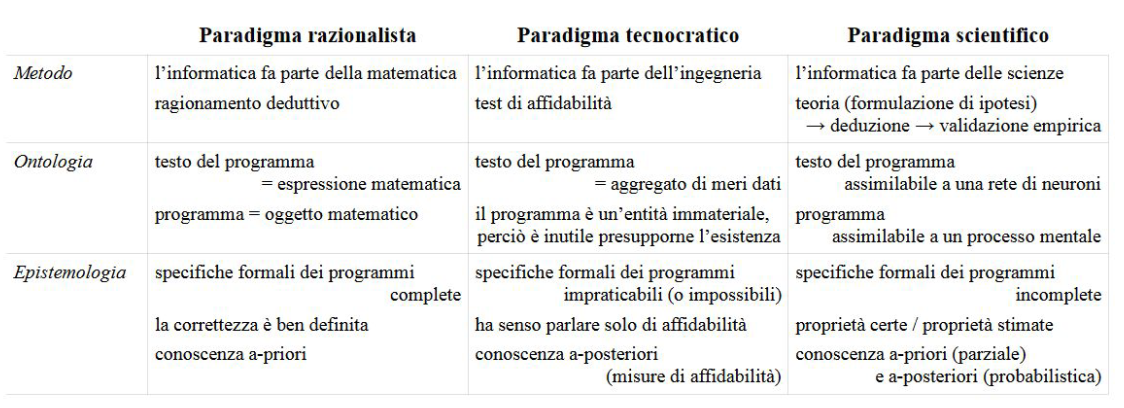
\includegraphics[scale = 0.4]{images/introduzione/Paradigmi.png}
\end{center}


\dfn{Paradigma razionalista (o matematico)}{Per il \newfancyglitter{paradigma razionalista} si  formalizza un linguaggio che garantisce certe proprietà (il tutto prima dell'esecuzione).}

\dfn{Paradigma tecnocratico (o ingegneristico)}{Per il \newfancyglitter{paradigma tecnocratico} si devono fare molti test di affidabilità con diversi input (unit test, a run time).}

\dfn{Paradigma scientifico}{Per il \newfancyglitter{paradigma scientifico} si deve validare empiricamente la correttezza di un programma.}
\subsubsection{}
Ognuno di questi paradigmi può essere usato per offrire una visione differennte dell'informatica:

\begin{itemize}
    \item alcune attività sono principalmente scientifiche: \evidence{algoritmi sperimentali};
    \item alcune attività sono principalmente ingegneristiche: \evidence{design}, \evidence{sviluppo}, etc;
    \item alcune attività sono principalmente matematiche: \evidence{calcolo di complessità}, \evidence{metodi formali}.
\end{itemize}

\paragraph{Perchè è importante pensarci?}

È importante pensare al prioprio modo di vedere l'informatica perchè ciò andrà a in cui si andrà a insegnare. Come si è visto la risposta è che l'informatica contiene in sè un po' di ogni paradigma, ma ci sono parti che possono essere ritenute, personalmente, più importanti.

\dfn{Anima matematica}{Rimanda al razionalismo filosofico. La \glitter{conoscenza pura} è più affidabile dei propri sensi (\glitter{conoscenza a posteriori}). L'unica metodologia accettabile è il ragionamento deduttivo. Il testo di un programma è un'espressione matematica.}

\dfn{Anima ingegneristica}{Rimanda all'empirismo inglese per cui l'esperienza è la base della conoscenza. È impossibile stabilire una conoscenza a priori sui programmi, l'informatica teorica è pura speculazione. Il metodo per valutare la qualità di un programma è il \glitter{testing} (abbinato alla statistica). Il testo di un programma è un aggregato di dati.}

\dfn{Anima scientifica}{Rimanda al metodo scientifico sperimentale. Si effettuano dei test basandosi su delle ipotesi. Il testo di un programma è assimilato a un \glitter{processo biologico} e la sua istanziazione (esecuzione) è assimilata a un \glitter{processo mentale}.}

\ex{Un algoritmo di ordinamento spiegato in una scuola secondaria di secondo grado}{
Un algoritmo di ordinamento può essere presentato in modi diversi a seconda dell'approccio scelto.

\evidence{Domande matematiche:}
\begin{itemize}
    \item L'algoritmo riesce a ordinare qualsiasi sequenza di dati, a prescindere dalla situazione iniziale, con eventuali ripetizioni?
    \item Gli algoritmi sono tutti uguali o ce ne sono di più efficienti?
    \item C'è un limite oltre cui non esiste un algoritmo pù veloce?
\end{itemize}

\evidence{Domande scientifiche:}
\begin{itemize}
    \item Come si possono misurare sperimentalmente i tempi di calcolo e con quale attendibilità?
    \item I tempi confermano i risultati teorici?
    \item Quali aspetti sono generali e quali contingenti?
    \item Quick Sort è sempre meglio di Insertion Sort?
\end{itemize}

\evidence{Domande ingegneristiche:}
\begin{itemize}
    \item È possibile migliorare le prestazioni di un algoritmo?
    \item Come si organizza il processo di sviluppo?
    \item Quali sono le condizioni ottimali?
\end{itemize}

}

\section{Quali sono i criteri per definire una scienza?}

\begin{itemize}
    \item Organizzata per capire, sfruttare e affrontare fenomeni pervasivi;
    \item Include sia processi naturali che artificiali;
    \item Ha un corpo ben strutturato;
    \item C'è un impegno per la scoperta e validazione dei principi;
    \item I risultati ottenuti sono riproducibili;
    \item Si possono falsificare ipotesi e modelli;
    \item Si riescono a fare ipotesi affifdabili, alcune sorprendenti.
\end{itemize}
